\section{Introduction}
    
    \begin{frame}
        
        \begin{center}
            \huge{Introduction}
        \end{center}
        
    \end{frame}
    
    \begin{frame}
        \frametitle{Historique}
        \begin{block}{À propos}
            Pong est un des premiers jeux vidéo d'arcade et le premier jeu vidéo d'arcade de sport. \\
            ~\\
            Commercialisé à partir de novembre 1972, il a été le premier jeu vidéo à devenir populaire. \\ %(8 000 d'exemplaires la première année et 40 millions de dollars de chiffres d'affaires en 1975)
            ~\\
            Le jeu est inspiré du tennis de table en vue de dessus.
        \end{block}
        
    \end{frame}
    
    \begin{frame}
        \frametitle{Représentation}
        \begin{figure}[h]
            \centering
            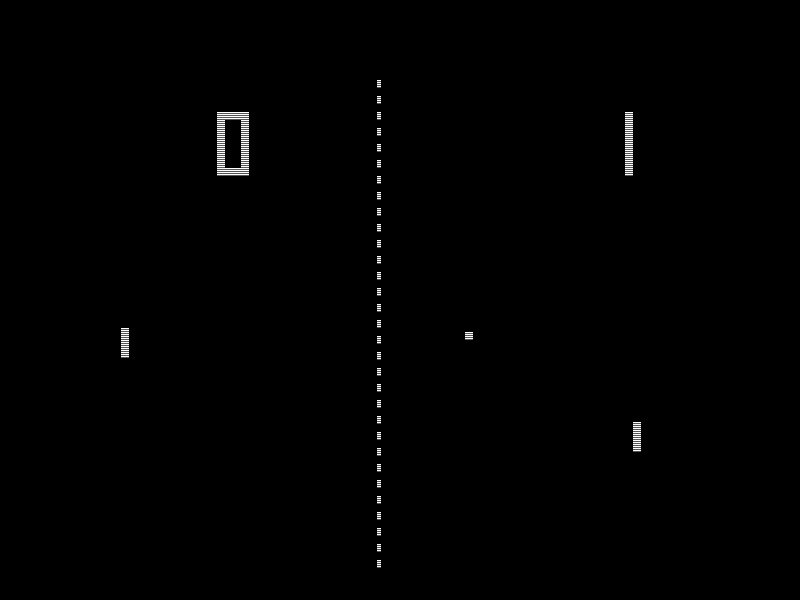
\includegraphics[scale=0.35]{images/intro/pong.png}
            \caption{Pong}
        \end{figure}
    \end{frame}
    
    \begin{frame}
        \frametitle{Raspberry Pi}
        \begin{block}{À propos}
            Basé sur le micro-contrôleur \textit{Atmel ATmega 644} dans ses premiers concepts, le Raspberry est un nano-ordinateur équipé d'un microprocesseur ARM. \\
            ~\\
            Debian \og \textit{jessie} \fg\ est recommandée par la fondation Raspberry Pi avec sa version dédiée \textbf{Raspbian}.
        \end{block}
        
    \end{frame}
    
    \begin{frame}
        \frametitle{Illustration}
        \begin{figure}[h]
            \centering
            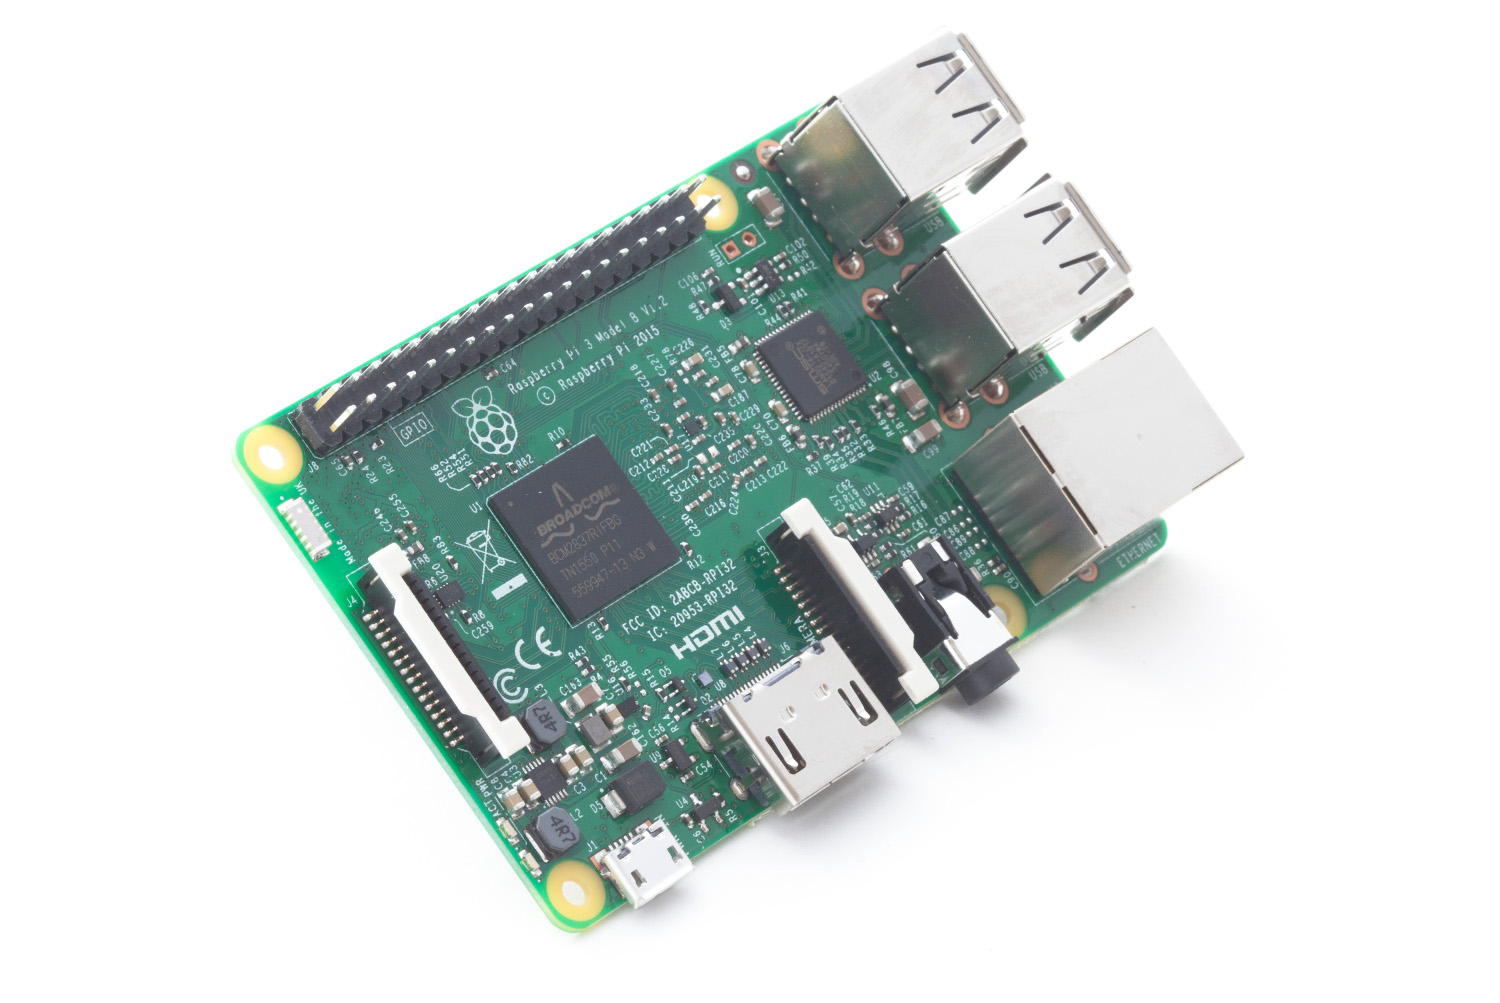
\includegraphics[scale=0.16]{images/intro/raspberry.jpg}
            \caption{Raspberry Pi- Modèle 3 B}
        \end{figure}
    \end{frame}
    
    \begin{frame}
        \frametitle{Sense HAT}
        \begin{block}{À propos}
            Le Sense HAT est une carte additionnelle disposant d’une matrice LED 8x8, d’un joystick et de nombreux capteurs. \\
            ~\\
            Il a été spécialement conçu pour la mission Astro Pi lancée en décembre 2015.
        \end{block}
        
    \end{frame}
    
    \begin{frame}
        \frametitle{Illustration}
        \begin{figure}[h]
            \centering
            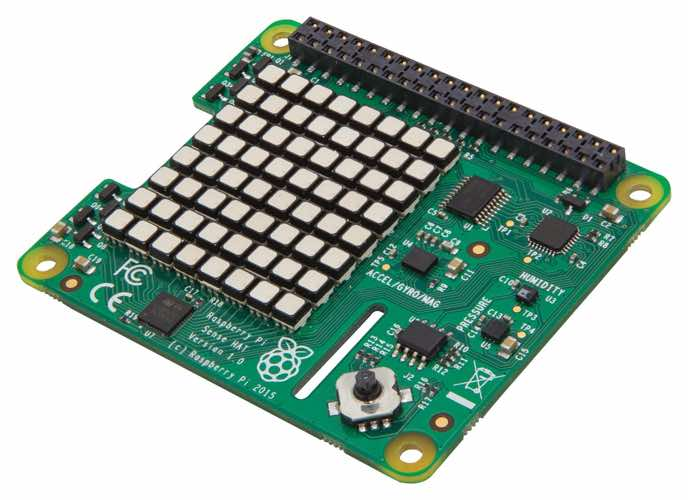
\includegraphics[scale=0.3]{images/intro/senseHAT.jpg}
            \caption{Sense HAT}
        \end{figure}
    \end{frame}